% !TEX root = coatli.tex

\chapter{The Huitzi $f/20$ Imager}

The Huitzi $f/20$ imager was installed on the COATLI telescope in December 2022. The imager is named for the mexica god \href{https://en.wikipedia.org/wiki/Huītzilōpōchtli}{Huītzilōpōchtli}, the son of the goddess Coatlicue.

Earlier, the “Interim Imager” and “Huitzi $f/8$ Imager” were installed on the telescope. For historical reference, these are described in Appendices~\ref{appendix:interim-imager} and \ref{appendix:instrument-huitzi-f8}.

\section{Overview}

\begin{figure}
\begin{center}
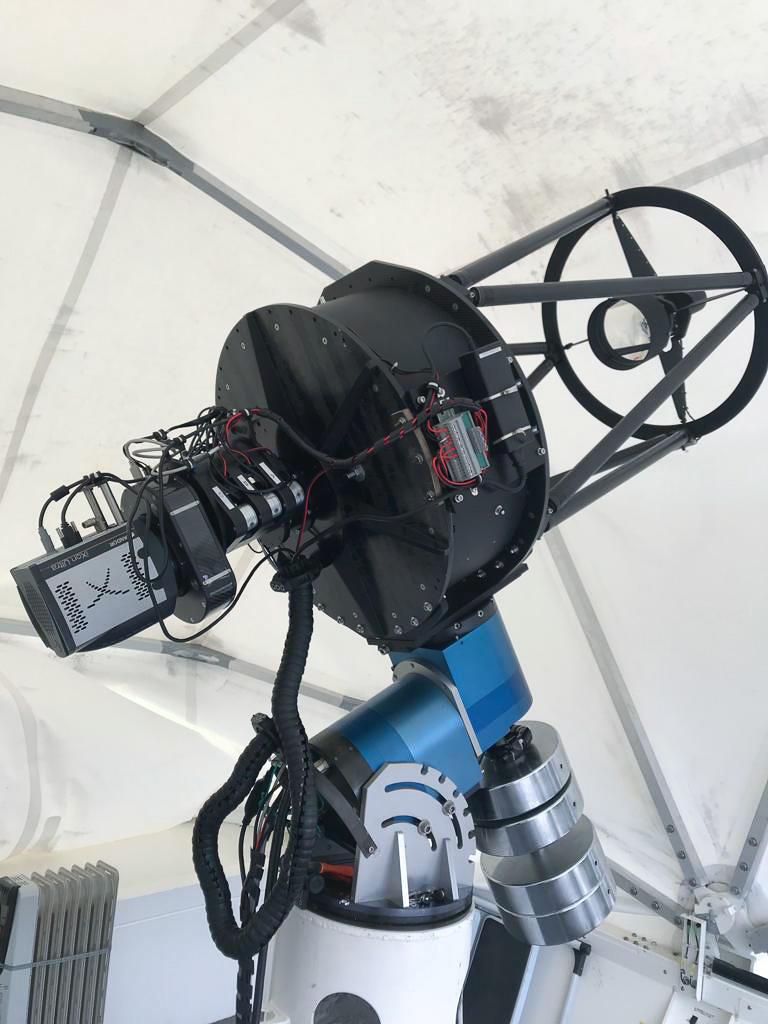
\includegraphics[width=0.7\linewidth]{figures/huitzi-on-telescope.jpg}
\medskip
\caption{The Huitzi $f/20$ imager on the COATLI telescope.}
\label{figure:huitzi-on-coatli}
\end{center}
\end{figure}

Figure~\ref{figure:huitzi-on-coatli} shows the Huitzi $f/20$ imager on the telescope.

The imager uses a 150 mm diverging lens to convert the $f/8$ beam of the telescope into an $f/20$ beam. This beam is then imaged an Andor iXon electron-multiplying CCD detector with $1024\times1024$ pixels with a pixel scale of 0.27 arcsec and a field of 4.6 arcmin. The detector can be read through either a conventional amplifier or the electron-multiplying amplifier at a variety of speeds.

The imager has three Finger Lakes Instruments filter wheels. Currently, the following filters can be provided:

\begin{itemize}
\item open: Completely open.
\item dark: Completely blocked.
\item $grizy$: Filters similar to the Pan-STARRS equivalents. Note, however, that while the filters are similar, the CCD is not deep-depleted and so the bandpasses are somewhat different.
\item $w$: A filter that combines the $r$ and $i$ bands. Note that this is different to Pan-STARRS $w$ which includes the $g$ band too. It is mainly intended for sensitive imaging of GRBs.
\item $BVRI$: Johnson-Cousins filters according to the Bessell formulation.
\item $\Is$: The $I$ filter with a sharp red cutoff at 900 nm. This is intended to better match the bandpass of the original Cousins (1978) $I$ photomety. The blue edge is the same as the Bessell formulation, but the red edge is defined by a 900 nm short-pass filter to simulate the red edge of a GaAs tube. The Bessell (1990) and Bessell \& Murphy (2012) bandpasses fall at about 900 nm.
\item 470/10, 515/10, and 640/10: Nebular continuum filters.
\item 501/8, 656/3, 656/8: Nebular line filters.
\end{itemize}

Some of these filters are constructed from combinations of filters in different wheels, as described in more detail below.

The detector is mounted on Optec Gemini focuser and rotator, which allows up to 12.7 mm of motion of the detector with respect to the lens.

\section{Optics}

\begin{figure}
\resizebox{\columnwidth}{!}{
\begin{tikzpicture}
\draw[dashed](-10,0) -- (12,0);
\draw(-8,+2) -- (-4,+1);
\draw(-8,-2) -- (-4,-1);
\draw[dotted](-4,+1) -- (0,0) -- (-4,-1);
\draw[>-<] (-4,-2) -- (-4,+2);
\draw (-4,+1) -- (10,0) -- (-4,-1);
\draw (-4,-2.5) node {$S$};
\draw (0,-2.5) node {$A$};
\draw (10,-2.5) node {$A'$};
\end{tikzpicture}
}
\medskip
\caption{Schematic of the Optical Design}
\label{figure:optical-design}
\end{figure}

The effect of the negative lens is shown schematically in Figure~\ref{figure:optical-design}. $A$ is the position of the telescope focus without the lens. $S$ is the position of the lens. $A'$ is the position of the telescope focus with the lens. 
The magnification $m$ is given by
$$
	m = SA'/SA,
$$
in which $SA'$ and $SA$ are optical distances.
If the focal length of the lens is $F$, then Gauss’ equation gives the relation between $SA$ and $SA'$ as:
$$
	1/F = 1/SA' - 1/SA.
$$
We then solve to find:
$$
	m = 1 - SA'/F
$$
and
$$
	SA' = - (m - 1) F.
$$
We can see the approximate dimensions of the system by ignoring chromatic aberration and taking $F = -150$ mm. Then, if we choose $SA = 90$ mm we have $SA' = 225$ mm and $m = 2.5$. Since the focal ratio of the telescope is $f/8$, this magnification gives a focal ratio of $f/20$.

\begin{figure}
\begin{center}
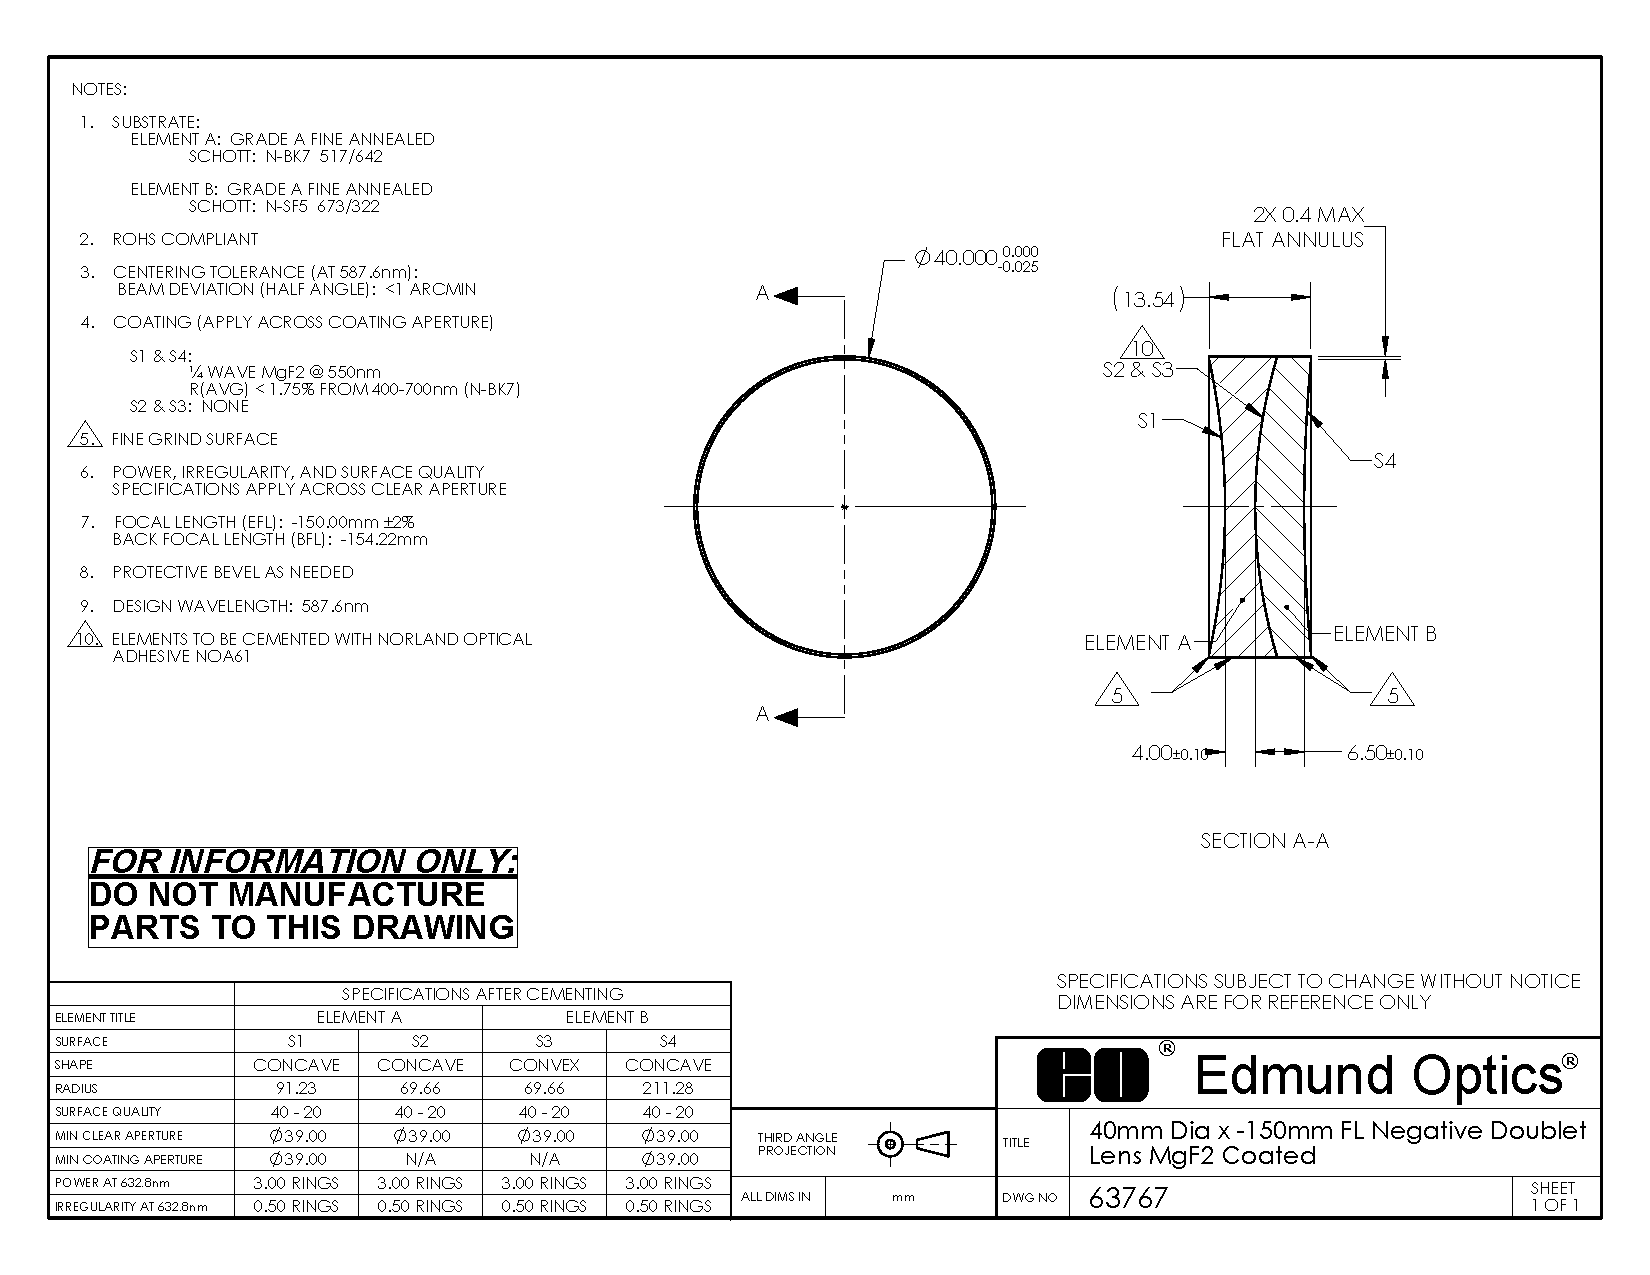
\includegraphics[width=0.8\linewidth]{figures/huitzi-lens-design.pdf}
\medskip
\caption{The lens design.}
\label{figure:huitzi-lens-design}
\end{center}
\end{figure}

The actual lens is Edmund Optics part \#63-767, whose design is shown in Figure~\ref{figure:huitzi-lens-design}. It has a design effective focal length of $-150$ mm at 587.6 nm. It is nominally 40 mm in diameter and 13.54 mm thick at the edge. The precise optical and mechanical prescriptions of are given in the files “\verb|zmax_63767.ZMX|”and “\verb|step_63767.STP|” supplied by Edmund Optics. The lens is used with the convergent element B uppermost (towards the secondary) and the divergent element A lowermost (towards the detector). That is, surface S4 is uppermost (towards the secondary) and surface S1 is lowermost (towards the detector). If the lens is inverted, the system will suffer significant spherical aberration.

The lens is an achromatic doublet, so its focal length varies with wavelength. This has two effects. First, the different focal length between bands requires us to refocus for each filter. In theory, we could adjust both the secondary and the focuser to achieve focus while holding the magnification constant. In practice, we simply adjust the focuser to maintain focus and let the magnification vary slightly. (The focuser is also used to compensate for the different optical thicknesses of the filters.) Second, chromatic aberration within the $g$ and $B$ bands limits their image quality.

The lens has a $\lambda/4$ MgF$_2$ coating on both surfaces.

The lens also serves as a window to prevent ingress of dust and insects.

\section{Filters}

The upper filter wheel (“A”) is an FLI CFW-1-5 wheel for five 50 mm diameter filters. The two lower filter wheels (“B” and “C”) are FLI CFW-1-8 wheels for eight 25 mm diameter filters. The elements installed in each wheel are shown in Table~\ref{table:filter-wheel-loading}.

\begin{table}
\begin{center}
\caption{Filter Wheel Loading}
\label{table:filter-wheel-loading}
\medskip
\begin{tabular}{llll}
\hline
Slot&A&B&C\\
\hline
0&open	&P0			&open		\\
1&$B$	&656/3		&$g$		\\
2&$V$	&470/10		&$r$		\\
3&$R$	&$z$			&$i$		\\
4&825SP	&$I$			&550LP	\\
5&			&925LP		&900SP	\\
6&			&515/10		&656/8	\\
7&			&640/10		&501/8	\\
\hline
\end{tabular}
\end{center}
\end{table}

The filter elements are:

\begin{itemize}
\item $griz$: These are similar to the Pan STARRS filters. They were acquired from Custom Scientific and fabricated to our specifications. They are 25 mm in diameter and 5 mm thick. They have dielectric coatings on fuzed silica substrates.
\item $BVRI$: These are Johnson-Cousins filters adapted from the Bessell (1990) recipe. They are off-the-shelf filters acquired from Custom Scientific. They are 50 mm ($BVR$) or 25 mm ($I$) diameter and 5 mm thick.
From modeling the transmission curves, we believe the recipes are:
\begin{itemize}
\item $B$: 2 mm Hoya L38 + 1 mm Schott BG25 + 2 mm Schott BG39
\item $V$: 1 mm Schott GG495 + 3 mm Schott BG39 + 1 mm filler
\item $R$: 2 mm Schott OG570 + 3 mm Schott KG3
\item $I$: 3 mm Schott RG9 + 2 mm filler
\end{itemize}
\item 825SP: This is an 825 nm OD4 short-pass filter. It is Edmund Optics part \#86-113. It is 50 mm in diameter and 5 mm thick. It has  dielectric coatings on a fuzed silica substrate.
\item 925LP: This is an 925 nm OD4 long-pass filter. It is Edmund Optics part \#86-072. It is 25 mm in diameter and 3 mm thick. It has  dielectric coatings on a fuzed silica substrate.
\item 900SP: This is an 900 nm OD4 short-pass filter. It is Edmund Optics part \#64-335. It is 25 mm in diameter and 3 mm thick. It has  dielectric coatings on a fuzed silica substrate.
\item 550LP: This is an 550 nm OD4 long-pass filter. It is Edmund Optics part \#62-984. It is 25 mm in diameter and 3 mm thick. It has dielectric coatings on a fuzed silica substrate.
\item P0: This is a window. It is Edmund Optics part \#48-066. It is 25 mm in diameter and 3 mm thick. It has Edmund UV-VIS coatings on a fused silica substrate.
\item 470/10, 501/8, 515/10, 640/10, 656/3, and 656/8: These are narrow-band filters, named for their approximate central wavelength and width in nm. They are off-the-shelf filters acquired from Custom Scientific. They are 25 mm in diameter and 3 mm thick. They have dielectric coatings on a fuzed silica substrate.

In addition to these, we have 486/8 and 501/3 filters that could be installed by special request. Furthermore, Custom Scientific have 672/3, 672/8, and 889/18 filters that could be purchased for about US\$500 each.
\end{itemize}

\begin{table}
\begin{center}
\caption{Filter Combinations}
\label{table:filter-combinations}
\medskip
\begin{tabular}{lllll}
\hline
Filter&A&B&C&Thickness (mm)\\
\hline
dark		&$B$		&$z$		&656/8	&\phantom{}13		\\
open		&open		&P0		&open		&\phantom{0}3		\\
$g$		&open		&P0		&$g$		&\phantom{0}8		\\
$r$		&open		&P0		&$r$		&\phantom{0}8		\\
$i$			&open		&P0		&$i$		&\phantom{0}8		\\
$z$		&open		&$z$		&open		&\phantom{0}5		\\
$y$		&open		&925LP	&550LP	&\phantom{0}6		\\
$w$		&825SP	&P0		&550LP	&\phantom{}11		\\
$B$		&$B$		&P0		&open		&\phantom{0}8		\\
$V$		&$V$		&P0		&open		&\phantom{0}8		\\
$R$		&$R$		&P0		&open		&\phantom{0}8		\\
$I$		&open		&$I$		&open		&\phantom{0}5		\\
$\Is$		&open		&$I$		&900SP	&\phantom{0}8		\\
470/10	&open		&470/10	&open		&\phantom{0}3		\\
501/8		&open		&P0		&501/8	&\phantom{0}6		\\
515/10	&open		&515/10	&open		&\phantom{0}3		\\
640/10	&open		&640/10	&open		&\phantom{0}3		\\
656/3		&open		&656/3	&open		&\phantom{0}3		\\
656/8		&open		&P0		&656/8	&\phantom{0}6		\\
\hline
\end{tabular}
\end{center}
\end{table}

The filter bandpasses are created by combinations of conventional bandpass filters, long-pass, and short-pass filters. The combinations used are given in Table~\ref{table:filter-combinations}. Most of the combinations are straightforward, but we comment on three aspects in particular:

\begin{itemize}
\item $\Is$: The system responses in both $I$ and $\Is$ have their blue edge defined by RG9 glass. However, in $I$ the red edge is defined by the CCD but in $\Is$ (“$I$ short”) it is defined by the 900SP filter. This gives $\Is$ a system response that is a better match that of Cousins (1978), whose $I$ has its the red edge defined by the cutoff of a GaAs photocathode around 900 nm. Compare Figure~\ref{figure:huitzi-S-JC-IIs} here with Figure~9 of Bessell \& Murphy (2012).

\item
$w$: The $w$ filter essentially encompasses the bandpasses of $r$ and $i$ (although the exact edges are slightly different). Note that this is different to Pan-STARRS $w$ which includes the $g$ band too. It is mainly intended for sensitive imaging of GRBs.

\item P0: The role of the P0 (“prism 0”) element might seem to be a puzzle. However, we are considering converting the telescope to an altitude-azimuth configuration at some point in the future and installing wedged windows P1 and P2, similar to P0, in wheel B in place of two of the narrow-band filters. This will allow us to implement an atmospheric dispersion corrector  for the $BVR$ and $griw$ filters using P0, P1, and P2. However, while the telescope is in an equatorial configuration, there is no point in installing P1 and P2. We could have left the position occupied by P0 as open, but we decided to install it to give consistent bandpasses in these filters in both the equatorial and altitude-azimuth configurations.

\end{itemize}

Model system efficiency curves at the zenith (including the atmosphere, telescope mirrors, lens, filters, detector window, and detector, but excluding the obscuration of the secondary) are shown in Figures~\ref{figure:huitzi-S-first} to \ref{figure:huitzi-S-last}.

\begin{figure}
\begin{center}
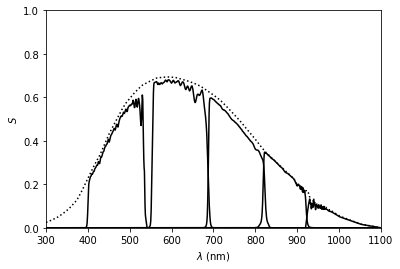
\includegraphics[width=0.9\linewidth]{figures/huitzi-S-grizy.png}
\medskip
\caption{The model system efficiency $S$ at the zenith in the $grizy$ filters. The dotted line is the model unfiltered efficiency.}
\label{figure:huitzi-S-first}
\end{center}
\medskip
\begin{center}
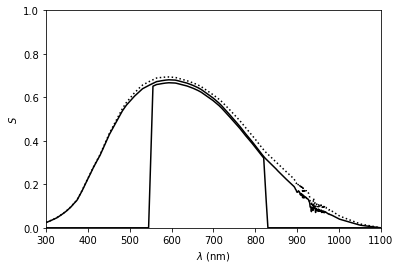
\includegraphics[width=0.9\linewidth]{figures/huitzi-S-w-open.png}
\medskip
\caption{The model system efficiency $S$ at the zenith in the $w$ and open filters. The dotted line is the model unfiltered efficiency.}
\end{center}
\end{figure}

\begin{figure}
\begin{center}
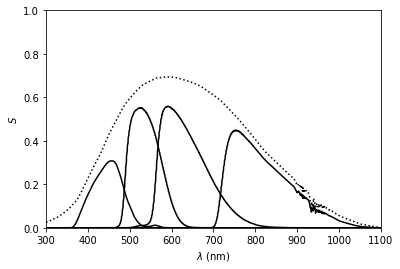
\includegraphics[width=0.9\linewidth]{figures/huitzi-S-JC-BVRI.png}
\medskip
\caption{The model system efficiency $S$ at the zenith in the $BVRI$ filters. The dotted line is the model unfiltered efficiency.}
\end{center}
\begin{center}
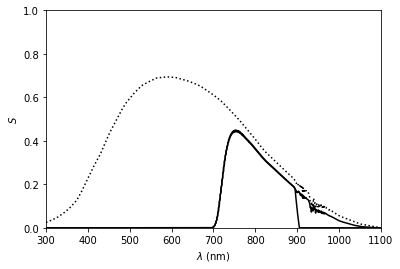
\includegraphics[width=0.9\linewidth]{figures/huitzi-S-JC-IIs.png}
\medskip
\caption{The model system efficiency $S$ at the zenith in the $I$ and $\Is$ filters. The $\Is$ filter has a red cutoff defined by the 900SP filter whereas the $I$ filter has the red cutoff defined by the CCD. The dotted line is the model unfiltered efficiency.}
\label{figure:huitzi-S-JC-IIs}
\end{center}
\end{figure}

\begin{figure}
\begin{center}
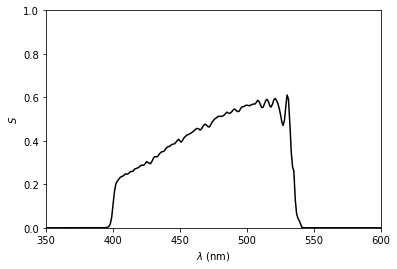
\includegraphics[width=0.9\linewidth]{figures/huitzi-S-g.png}
\medskip
\caption{The model system efficiency $S$ at the zenith in the $g$ filter.}
\end{center}
\end{figure}

\begin{figure}
\begin{center}
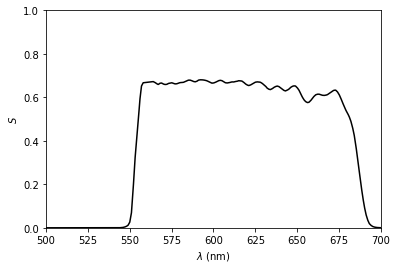
\includegraphics[width=0.9\linewidth]{figures/huitzi-S-r.png}
\medskip
\caption{The model system efficiency $S$ at the zenith in the $r$ filter.}
\end{center}
\end{figure}

\begin{figure}
\begin{center}
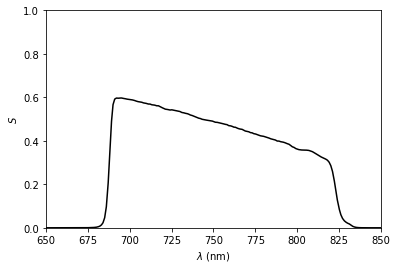
\includegraphics[width=0.9\linewidth]{figures/huitzi-S-i.png}
\medskip
\caption{The model system efficiency $S$ at the zenith in the $i$ filter.}
\end{center}
\end{figure}

\begin{figure}
\begin{center}
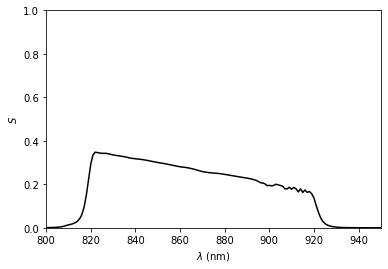
\includegraphics[width=0.9\linewidth]{figures/huitzi-S-z.png}
\medskip
\caption{The model system efficiency $S$ at the zenith in the $z$ filter.}
\end{center}
\end{figure}

\begin{figure}
\begin{center}
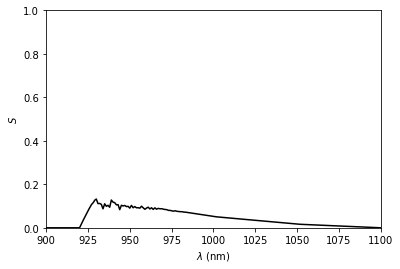
\includegraphics[width=0.9\linewidth]{figures/huitzi-S-y.png}
\medskip
\caption{The model system efficiency $S$ at the zenith in the $y$ filter.}
\end{center}
\end{figure}

\begin{figure}
\begin{center}
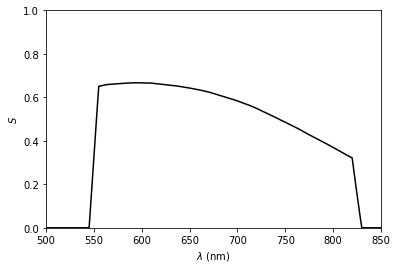
\includegraphics[width=0.9\linewidth]{figures/huitzi-S-w.png}
\medskip
\caption{The model system efficiency $S$ at the zenith in the $w$ filter.}
\end{center}
\end{figure}

\begin{figure}
\begin{center}
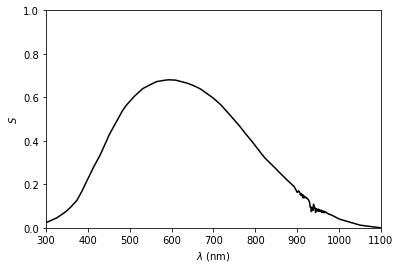
\includegraphics[width=0.9\linewidth]{figures/huitzi-S-open.png}
\medskip
\caption{The model system efficiency $S$ at the zenith in the open filter.}
\end{center}
\end{figure}

\begin{figure}
\begin{center}
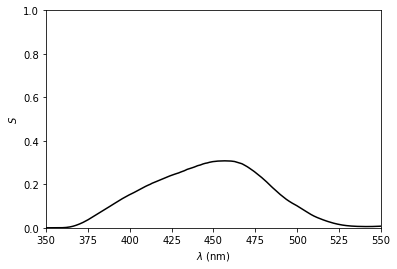
\includegraphics[width=0.9\linewidth]{figures/huitzi-S-JC-B.png}
\medskip
\caption{The model system efficiency $S$ at the zenith in the $B$ filter.}
\end{center}
\end{figure}

\begin{figure}
\begin{center}
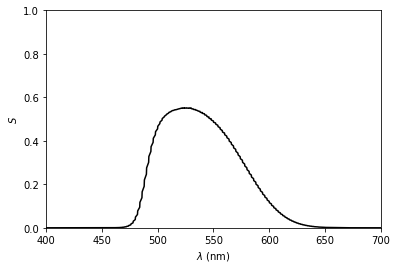
\includegraphics[width=0.9\linewidth]{figures/huitzi-S-JC-V.png}
\medskip
\caption{The model system efficiency $S$ at the zenith in the $V$ filter.}
\end{center}
\end{figure}

\begin{figure}
\begin{center}
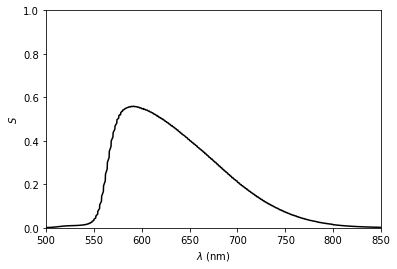
\includegraphics[width=0.9\linewidth]{figures/huitzi-S-JC-R.png}
\medskip
\caption{The model system efficiency $S$ at the zenith in the $R$ filter.}
\end{center}
\end{figure}

\begin{figure}
\begin{center}
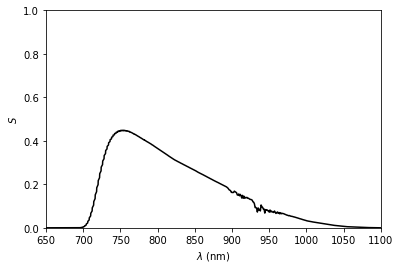
\includegraphics[width=0.9\linewidth]{figures/huitzi-S-JC-I.png}
\medskip
\caption{The model system efficiency $S$ at the zenith in the $I$ filter.}
\end{center}
\end{figure}

\begin{figure}
\begin{center}
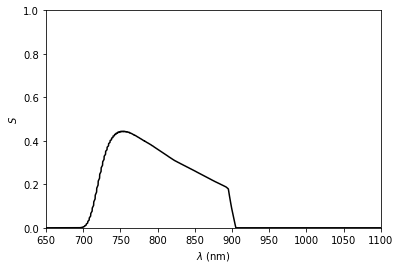
\includegraphics[width=0.9\linewidth]{figures/huitzi-S-JC-Is.png}
\medskip
\caption{The model system efficiency $S$ at the zenith in the $\Is$ filter.}
\end{center}
\end{figure}

\begin{figure}
\begin{center}
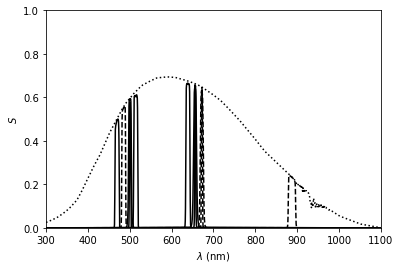
\includegraphics[width=0.9\linewidth]{figures/huitzi-S-NBMB.png}
\medskip
\caption{The model system efficiency $S$ at the zenith in the narrow-band and medium-band filters. The dotted line is the model unfiltered efficiency.}
\end{center}
\end{figure}

\begin{figure}
\begin{center}
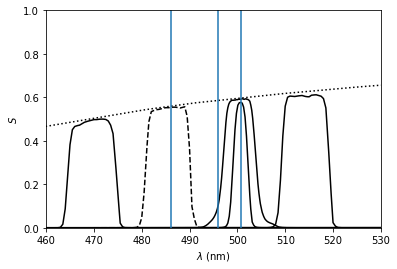
\includegraphics[width=0.9\linewidth]{figures/huitzi-S-NBMB-g.png}
\medskip
\caption{The model system efficiency $S$ at the zenith in the narrow-band and medium-band filters in $g$: 470/10, 486/8, 501/3, 501/8, and 515/10. The filters shown with dashed lines have not yet been acquired. The dotted line is the model unfiltered efficiency. The blue vertical lines are at 486.1, 495.9, and 500.7 nm.}
\end{center}
\end{figure}

\begin{figure}
\begin{center}
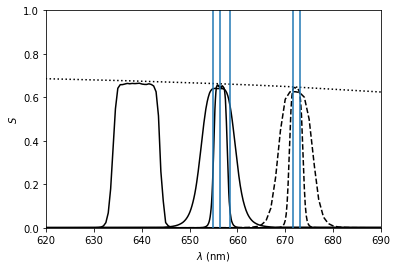
\includegraphics[width=0.9\linewidth]{figures/huitzi-S-NBMB-r.png}
\medskip
\caption{The model system efficiency $S$ at the zenith in the narrow-band and medium-band filters in $r$: 640/10, 656/3, 656/8, 672/3, and 672/8, 501/8, and 515/10. The filters shown with dashed lines have not yet been acquired. The dotted line is the model unfiltered efficiency. The blue vertical lines are at 656.3, 654.8, 658.4, 671.6, and 673.1 nm.}
\end{center}
\end{figure}

\begin{figure}
\begin{center}
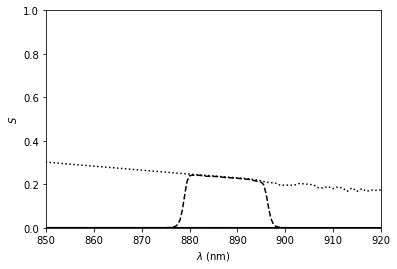
\includegraphics[width=0.9\linewidth]{figures/huitzi-S-NBMB-z.png}
\medskip
\caption{The model system efficiency $S$ at the zenith in the medium-band filter in $z$: 889/18. The filters shown with dashed lines have not yet been acquired. The dotted line is the model unfiltered efficiency.}
\label{figure:huitzi-S-last}
\end{center}
\end{figure}

\begin{table}
\begin{center}
\caption{Model Filter Properties}
\label{table:model-filter-properties}
\medskip
\begin{tabular}{lccc}
\hline
Filter&$\lambda_\mathrm{pivot}$ (nm)&$\Delta\lambda$ (nm)&ZP ($\mathrm{s}^{-1}$)\\
\hline
open		& 618.7& \phantom{}384.1&$4.2 \times 10^{9}$\\
$g$		& 475.9& \phantom{}104.6&$1.2 \times 10^{9}$\\
$r$		& 617.2& \phantom{}132.4&$1.3 \times 10^{9}$\\
$i$			& 747.4& \phantom{}131.5&$8.0 \times 10^{8}$\\
$z$		& 862.8& \phantom{0}94.8&$3.0 \times 10^{8}$\\
$y$		& 973.3& \phantom{0}64.2&$8.6 \times 10^{7}$\\
$w$		& 668.4& \phantom{}264.6&$2.2 \times 10^{9}$\\
$B$		& 446.5& \phantom{0}89.4&$5.9 \times 10^{8}$\\
$V$		& 537.9& \phantom{0}89.8&$8.5 \times 10^{8}$\\
$R$		& 633.9& \phantom{}118.0&$1.0 \times 10^{9}$\\
$I$		& 814.8& \phantom{}150.7&$8.0 \times 10^{8}$\\
$\Is$		& 795.0& \phantom{}150.7&$7.0 \times 10^{8}$\\
470/10	& 469.7& \phantom{0}10.1&$9.9 \times 10^{7}$\\
486/8		& 485.5& \phantom{00}9.3&$1.0 \times 10^{8}$\\
501/3		& 500.7& \phantom{00}3.2&$3.5 \times 10^{7}$\\
501/8		& 500.5& \phantom{00}7.0&$8.2 \times 10^{7}$\\
515/10	& 514.2& \phantom{0}10.0&$1.1 \times 10^{8}$\\
640/10	& 638.9& \phantom{00}9.9&$9.8 \times 10^{7}$\\
656/3		& 656.5& \phantom{00}2.9&$2.8 \times 10^{7}$\\
656/8		& 655.9& \phantom{00}7.7&$8.4 \times 10^{7}$\\
672/3		& 672.3& \phantom{00}2.9&$2.7 \times 10^{7}$\\
672/8		& 672.2& \phantom{00}7.6&$6.8 \times 10^{7}$\\
889/18	& 887.3& \phantom{0}17.5&$4.3 \times 10^{7}$\\
\hline
\end{tabular}
\end{center}
\end{table}

Table~\ref{table:model-filter-properties} gives the model properties of the filter. The filter pivot wavelength $\lambda_\mathrm{pivot}$ is  defined by 
$$
\lambda_\mathrm{pivot} \equiv \sqrt{\frac{\int \lambda S\,d\lambda}{\int S/\lambda\, d\lambda}}.
$$
For a discussion of the interpretation of the pivot wavelength, see \S A2.1 of Bessell \& Murphy (2012).
The filter FWHM is defines as the width over which $S$ is at least half its maximum. The filter ZP is the expected electron count rate for a star with AB = 0,
$$
ZP \equiv A \int S F_\lambda / (hc/\lambda)\, d\lambda,
$$
in which $A$ is the geometric area of the telescope (the area of the primary mirror not occulted by the secondary obscuration) and $F_\lambda$ is the flux density of a source with $F_\nu = \mathrm{3631~Jy}$.

We are monitoring photometric standards from Oke \& Gunn (1983) to verify the theoretical zero-points and sensitivity curves presented above. Initial results suggest that the zero points in the blue are approximately correct, but beyond about 600 nm the observed sensitivity is only about 75\% of the theoretical sensitivity.

\section{Focuser and Rotator}

The instrument incorporates an Optec Gemini focuser and rotator between the last filter wheel and the detector.

The focuser moves from 0 to 115200 steps over 12.7 mm which corresponds to 9.07 steps per micron. The 0 position is above and the 115200 position is below. The focuser moves at about 900 steps or 0.1 mm per second.

\section{Focus Compensation}

The lens has chromatic aberration and the filters have different thicknesses. Both of these require us to use a compensator to maintain focus. Our options are the focuser, the secondary, or both. If we use only one compensator, then the magnification necessarily changes slightly was we adjust for focus. If we use both, we can maintain the magnification. 

However, it is fairly easy to show that if we use the focuser, either on its own or in combination with the secondary to maintain the magnification, in the worst case we need to move it about 3 mm. Since the focuser moves at about 0.1 mm per second, this means the worse case time is about 30 seconds. This is long compared to slew speed (without a meridian flip) and cannot be overlapped with changing the filter.  On the other hand, if we use only the secondary, in the worst case we need to move about 60 steps. Even with backlash compensation, this takes about 5.5 seconds. Furthermore, this can be overlapped with changing the filter. Therefore, in the interests of preserving the rapid response of COATLI, we have chosen to compensate the focus using only the secondary. This compensation is handled automatically by the control system.

Our model is as follows. We define $L$ to be the (fixed) physical distance from the lens to the detector and $T$ to be the total physical thickness of filter glass between the lens and the detector. We then have
$$
SA' = L - [(n - 1) / n] T \approx L - 0.32 T,
$$
where we have assumed $n = 1.48$ for fused silica. We then solve for SA using
$$
1/F = 1/SA' - 1/SA,
$$
taking into account the dependence of $F$ on wavelength. We determine $\Delta SA$ relative to the $i$ filter. We then determine the corresponding change in the secondary taking into account the amplification of 10.64 between the movement of the secondary and the movement of the telescope focal plane.

Table \ref{table:filter-secondary-offsets} shows the results. Note that for the medium band filters, there are two values depending on whether the filter is in wheel B ($T = 3$ mm) or wheel C ($T = 6$ mm). The offsets of the narrowband filters are the same as for the corresponding medium band filters.

\begin{table}
\begin{center}
\caption{Filter Secondary Offsets}
\label{table:filter-secondary-offsets}
\medskip
\begin{tabular}{lccc}
\hline
Filter&$F$ (mm)&Thickness (mm)&Offset (steps)\\
\hline
open		&$-150.22$		&\phantom{0}3		&\phantom{}$-24$\\
$g$		&$-150.20$		&\phantom{0}8		&\phantom{0}$+7$\\
$r$		&$-150.07$		&\phantom{0}8		&\phantom{}$+13$\\
$i$			&$-150.37$		&\phantom{0}8		&\phantom{+0}$0$\\
$z$		&$-150.66$		&\phantom{0}5		&\phantom{}$-30$\\
$y$		&$-150.96$		&\phantom{0}6		&\phantom{}$-37$\\
$w$		&$-150.25$		&\phantom{}11		&\phantom{}$+24$\\
$B$		&$-150.43$		&\phantom{0}8		&\phantom{0}$-2$\\
$V$		&$-150.97$		&\phantom{0}8		&\phantom{}$+17$\\
$R$		&$-150.14$		&\phantom{0}8		&\phantom{}$+10$\\
$I$		&$-150.27$		&\phantom{0}5		&\phantom{}$-30$\\
$\Is$		&$-150.50$		&\phantom{0}8		&\phantom{0}$-5$\\
470/10	&$-149.99$		&\phantom{}3/6		&\phantom{}$-14/+4$\\
515/10	&$-149.93$		&\phantom{}3/6		&\phantom{}$-12/+6$\\
640/10	&$-150.07$		&\phantom{}3/6		&\phantom{}$-16/+1$\\
\hline
\end{tabular}
\end{center}
\end{table}

\section{Detector}

The detector unit is an Andor iXon Ultra 888 with an e2v CCD201-20 electron-multiplying CCD detector. The detector was acquired in 2014 and originally intended to be the tilt sensor for the planned two-channel imager.

\subsection{Format, Scale, and Field}

The detector has $1024\times1024$ pixels each $13\times13$ {\micron} square. 

The detector gives a pixel scale of 0.269 arcsec and a field of 4.59 arcmin. 

\begin{figure}
\begin{center}
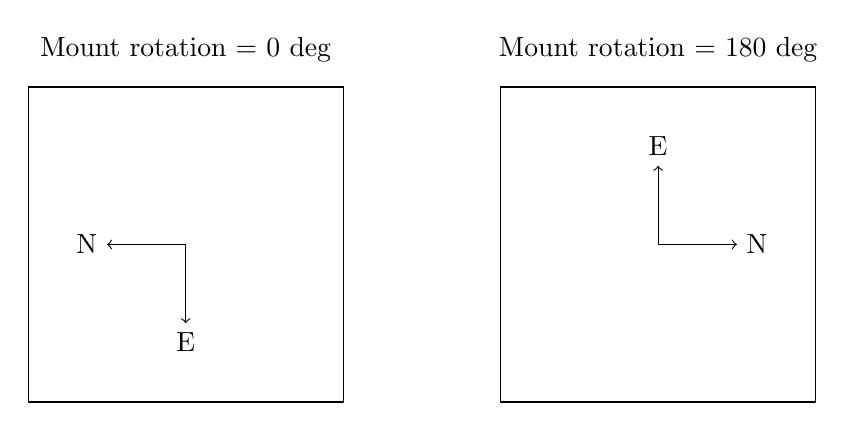
\begin{tikzpicture}
\begin{scope}[xshift=-3cm]
\draw (-2,-2) -- (+2,-2) -- (+2,+2) -- (-2,+2) -- cycle;
\draw (0,2.2) node [anchor=south] {Mount rotation = 0 deg};
\draw[->] (0,0) -- (-1,0) node [anchor=east] {N};
\draw[->] (0,0) -- (0,-1) node [anchor=north] {E};
\end{scope}
\begin{scope}[xshift=3cm]
\draw (-2,-2) -- (+2,-2) -- (+2,+2) -- (-2,+2) -- cycle;
\draw (0,2.2) node [anchor=south] {Mount rotation = 180 deg};
\draw[->] (0,0) -- (1,0) node [anchor=west] {N};
\draw[->] (0,0) -- (0,1) node [anchor=south] {E};
\end{scope}
\end{tikzpicture}
\end{center}
\caption{The orientation of the detector on the sky according to the mount rotation. The pixel origin is in the lower left.}
\label{figure:detector-orientation}
\end{figure}

The orientation of the field on the sky depends on the mount rotation (given by the values of the \verb|SMTMRO| and \verb|EMTMRO| keywords in the header), and is shown in Figure~\ref{figure:detector-orientation}. However, the pipeline reduction rotates all images to the conventional orientation with north up and east left.

\subsection{Quantum Efficiency}

The detector has standard silicon and the e2v midband coating (which in Andor's terminology makes it a “BV” device). The nominal quantum efficiency is shown in Figure~\ref{figure:detector-quantum-efficiency}. The detector has excellent efficiency from 500 to 800 nm.

\begin{figure}
\begin{center}
\begin{tikzpicture}
\small
\begin{axis}[
   xmin=300,
   xmax=1100,
   xlabel={$\lambda$ (nm)},
   xticklabel style={
     /pgf/number format/precision=0,
     /pgf/number format/fixed,
     /pgf/number format/fixed zerofill
   },
   minor x tick num=3,
   ymin=0,
   ymax=1,
   minor y tick num=3,
   ylabel={$\eta$},
   legend style={
     cells={anchor=west},
     legend pos=north east,
   },
]
\addplot [black] table [x=lam, y=Q, col sep=comma] {figures/huitzi-detector-efficiency.csv};
\end{axis}
\end{tikzpicture}
\end{center}
\caption{The nominal quantum efficiency $\eta$ of the Huitzi detector.}
\label{figure:detector-quantum-efficiency}
\end{figure}


\subsection{Readout Architecture}

The detector can be read using either a conventional signal chain (at 100 kHz or 1 MHz) or an EM signal chain (at 1, 10, 20, or 30 MHz). Both chains have two gains and the EM gain can be set to up to 1000. 

Although the conventional and EM amplifiers clock the serial register in different directions, the control software flips each row in conventional data so that physical pixels have the same logical position in the FITS files.

The detector is used in frame-transfer mode without a mechanical shutter (see \S\ref{section:shutter}). At the end of an exposure, the charge is rapidly clocked into from the light-sensitive image section to the shielded store section. The change can then be read. In EM mode, the next exposure can then start immediately.

With the normal vertical-shift frequency of 4.33 MHz, the frame transfer takes about 4.5 ms. This leads to some trailing above and below bright stars.

The read-out architecture has several parameters, which are encoded in the value of the \verb|READMODE| header keyword. The value is a string of the form $A$-$B$-$C$-$D$-$E$-$F$-$G$ in which $A$ to $G$ are non-negative integers with the following meanings:

\begin{itemize}
\item[$A$] The ADC channel index. This is always 0 since the detector only has one ADC channel.
\item[$B$] The amplifier index. This is 0 for the EM amplifier and 1 for the conventional amplifier.
\item[$C$] The vertical shift speed index. For both amplifiers, 0 is 0.60 MHz, 1 is 1.13 MHz, 2 is 2.20 MHz, and 3 is 4.33 MHz. 
\item[$D$] The horizontal shift speed index. For the EM amplifier, 0 is 30 MHz, 1 is 20 MHz, 2 is 10 MHz, and 3 is 1 MHz. For the conventional amplifier, 0 is 1 MHz and 1 is 100 kHz.
\item[$E$] The gain index. For both amplifiers, 0 is low gain (more electrons per ADU) and 1 is high gain (fewer electrons per ADU).
\item[$F$] The nominal EM gain. This is ignored when the conventional amplifier is used. For the EM amplifier, it can be between 1 and 1000.
\item[$G$] The software gain. After the data are read, each ADU signal is divided by the software gain to reduce white noise in the low-order bits (see \href{https://ui.adsabs.harvard.edu/abs/2002RMxAA..38..233W/abstract}{Watson 2002, RMAA, 38, 233}).
\end{itemize}

Fortunately, there is little need to use these values directly, since aliases are defined for common modes. They are shown in Table~\ref{table:read-mode-aliases}.

\begin{table}
\caption{Read-Mode Aliases}
\label{table:read-mode-aliases}
\begin{center}
\begin{tabular}{lll}
\hline
Alias&Mode\\
\hline
 initial&default\\
 default&em-30MHz\\
 conventionaldefault&1MHz\\
 fastguidingdefault&em-30MHz\\
 1MHz&1MHz-low\\
 em-10MHz&em-10MHz-low\\
 em-20MHz&em-20MHz-low\\
 em-30MHz&em-30MHz-low\\
 1MHz-low&0-1-3-0-0-1-1\\
 1MHz-high&0-1-3-0-1-1-2\\
 em-10MHz-low&0-0-3-2-0-250-2\\
 em-10MHz-high&0-0-3-2-1-160-4\\
 em-20MHz-low&0-0-3-1-0-500-4\\
 em-20MHz-high&0-0-3-1-1-320-8\\
 em-30MHz-low&0-0-3-0-0-1000-8\\
 em-30MHz-high&0-0-3-0-1-640-16\\
 \hline
\end{tabular}
\end{center}
\end{table}

\subsection{Shutter and Dark Filter}

\label{section:shutter}

We originally attempted to use the mechanical shutter for conventional CCD modes and the frame-transfer capability for EM modes. However, we found that the shutter sometimes failed to open or failed to open completely. We suspect that at the colder temperatures at night, the power supply does not provide sufficient voltage to open the shutter.  Therefore, we now leave the shutter open permanently and use the frame-transfer capability in both conventional and EM modes. As noted above, with the normal vertical-shift frequency, the frame transfer takes about 4.5 ms.

To take bias and dark images, we have use a “dark” filter that consists of the $B$, $z$, and 656/8 filters in series. Despite this, light leaks in the filter wheel mean that we need to take biases and darks at night.

\begin{table}
    \centering
    \begin{tabular}{lcccc}
    \hline
    Mode Name&1MHz-0&em-10MHz-0&em-20MHz-0&em-30MHz-0\\
    \hline
    Amplifier&Conventional&EM&EM&EM\\
    Horizontal Speed&1 MHz&10 MHz&20 MHz&30 MHz\\
    Software Gain&1&2&4&8\\
    ADC Range (DN)&64k&32k&16k&8k\\
    Gain ($e^-$/DN)&3.3&41&78&117\\
    Read Noise (DN)&2.1&2.6&1.9&1.7\\
    Read Noise ($e^-$)&7&105&145&204\\
    Bias Level (DN)&500&242&123&62\\
    Linear Limit ($e^-$)&&400k&400k&400k\\
    Saturation (DN)&58k&32k&16k&8k\\
    Saturation ($e^-$)&190k&1300k&1250k&940k\\
    Linearity ($e^-$)&&400k&400k&400k\\
    Linearity (DN)&&9700&5100&3400\\
    Dynamic Range (bits)&&11.9&11.4&10.9\\
    \hline
    \end{tabular}
    \caption{Detector Characteristics with the Low Preamplifier Gain}
    \label{table:detector-characteristics-low-gain}
\end{table}

\begin{table}
    \centering
    \begin{tabular}{lcccc}
    \hline
    Mode Name&1MHz-1&em-10MHz-1&em-20MHz-1&em-30MHz-1\\
    \hline
    Amplifier&Conventional&EM&EM&EM\\
    Horizontal Speed&1 MHz&10 MHz&20 MHz&30 MHz\\
    Software Gain&2&4&8&16\\
    ADC Range (DN)&32k&16k&8k&4k\\
    Gain ($e^-$/DN)&1.6&21&45&70\phantom{0}\\
    Read Noise (DN)&2.9&2.7&2.4&1.6\\
    Read Noise ($e^-$)&5&56&108&115\\
    Bias Level (DN)&250&119&62&31\\
    Saturation (DN)&22k&\\
    Saturation ($e^-$)&35k&\\
    Linearity ($e^-$)&&400k&400k&400k\\
    Linearity (DN)&&19000&8900&5700\\
    Dynamic Range (bits)&&12.8&11.9&11.8\\
    \hline
    \end{tabular}
    \caption{Detector Characteristics with the High Preamplifier Gain}
    \label{table:detector-characteristics-high-gain}
\end{table}



\section{Bibliography}

\begin{flushleft}
\begin{itemize}
\item “\href{bibliography/huitzi/andor-ixon-ultra-888-data-sheet.pdf}{Andor iXon Ultra 888 Data Sheet}”, Andor, May 2014.
\item “\href{bibliography/huitzi/andor-ixon-ultra-888-hardware-guide.pdf}{Andor iXon Ultra \& Life 888 Hardware Guide}”, Andor, Version 1.8 of 30 September 2019.
\item Bessell, M.S., 1990, PASP, 102, 1181: “$UBVRI$ Passbands”.
\item Bessell, M., \& Murphy, S., 2012,  PASP, 124, 140: “Spectrophotometric Libraries, Revised Photonic Passbands, and Zero Points for UBVRI, Hipparcos, and Tycho Photometry”.
\item “\href{bibliography/huitzi/e2v-ccd201-20-datasheet.pdf}{CCD201-20 Datasheet}”, Teledyne e2v, Version 7 of August 2019.
\item Cousins, A.W.J., 1976, MNRAS, 81, 25: “VRI standards in the E regions”.
\item Oke, J.B, \& Gunn, J.E., 1983, ApJ, 266, 713: “Secondary Standard Stars for Absolute Spectrophotometry”
\end{itemize}
\end{flushleft}


